\documentclass{article}
\usepackage{fancyvrb}
\usepackage{xcolor}
\usepackage{float}
\usepackage{graphicx}
\usepackage[utf8]{inputenc}

\title{Automação Em Tempo Real: Desafio}
\author{Gabriel Teixeira Lara Chaves\\
        2017088182}
        
\date{Janeiro de 2021}

\begin{document}

\maketitle

\section{Introdução}

O seguinte relatório tem por objetivo documentar a
solução proposta pelo autor para o desafio elaborado
em torno do problema de sincronização da barbearia.
O problema consiste em sincronizar a ação de três
barbeiros que atendem um número arbitrário de clientes.
A tarefa que deve ser sincronizada em si é o trabalho dos barbeiros, no qual um barbeiro
pode atender apenas um cliente por vez. Adicionalmente é requerido
pelo desafio que um dos três barbeiros operantes funcione também como caixa, recebendo o pagamento que
deve, necessariamente, ser feito por cada cliente após
ser atendido. Esse barbeiro que atua como caixa deve
receber os pagamentos enquanto não estiver atendendo clientes.

\section{Objetos de Sincronização}

Os objetos usados na sincronização são \textit{mutexes}, semáforos e variáveis globais.
Cada um será descrito a seguir, referenciado pelo nome de sua variável no código. Recomenda-se
que o código, que está devidamente comentado, seja lido antes de prosseguir neste documento.

\subsection{\textit{Mutexes}}

Apenas um \textit{mutex} nomeado \verb+look+ é utilizado no código. Esse \textit{mutex} assume função
de controlar acesso a variáveis globais de interesse dentro de uma mesma \textit{thread}, como o contador
global de número de clientes dentro da barbearia que será analisado em breve. 

\subsection{Semáforos}

Os semáforos usados na sincronização, assim como suas funções, serão listados a seguir:

\begin{itemize}
    \item \textbf{chair}: Controla acesso dos clientes às cadeiras dos barbeiros. Sinal é dado por um barbeiro e recebido por um cliente.
    \item \textbf{wake}: Controla atenção dos barbeiros aos clientes. Sinal é dado pelo cliente e recebido por um barbeiro. O barbeiro "acorda" para atender o cliente que o sinalizou.
    \item \textbf{end}: Controla permanência do cliente na cadeira conquistada. Sinal é dado pelo barbeiro ao terminar a barba do cliente e recebido pelo cliente.
    \item \textbf{leave\_chair}: Controla acesso dos clientes às cadeiras dos barbeiros. Garante que apenas um cliente fique em uma cadeira simultaneamente, evitando a situação constrangedora que resultaria do contrário. Sinal é dado pelo cliente após receber o sinal que o barbeiro terminou sua barba.
    \item \textbf{end\_pay}: Semáforo contador que será incrementado de acordo com o número de clientes que deseja pagar. Controla saída dos clientes de forma que eles tenham que esperar que o barbeiro-caixa receba seu dinheiro. Impede que clientes passem a perna na barbearia. Sinal é dado pelo barbeiro-caixa e recebido pelos clientes que aguardam o pagamento.
\end{itemize}

\subsection{Variáveis Globais}

\begin{itemize}
    \item \textbf{client\_counter}: Contador de quantos clientes há no estabelecimento. Necessário para determinar se um cliente entra ou volta para casa.
    \item \textbf{payers}: Contador de número de clientes que aguardam o barbeiro-caixa para pagar.
\end{itemize}

\section{Descrição da Solução}

O método apresentado funciona para qualquer número de clientes, barbeiros e barbeiros-caixa (em níveis variáveis de eficiência). Sua descrição será detalhada para os valores especificados no enunciado.

A proposta se basea na utilização de uma variável global (\verb+payers+) em conjunto com um semáforo (\verb+end_pay+) para coordenar a função dupla do babeiro-caixa. Emprega-se adicionalmente uma espera temporizada por parte do barbeiro-caixa para o pedido de acesso de um cliente à sua cadeira a fim evitar um \textit{deadlock} que resultaria de casos onde o número de clientes é próximo ou inferior ao número de barbeiros ou a lotação da barbearia é baixa. O código das \textit{threads} babeiro e
cliente será representado por meio de (pseudo)pseudocódigo a seguir para explicar a proposta. Para evitar redundância os trechos de código protegidos pelo \textit{mutex} empregado serão simplesmente destacados em vermelho. Mais atenção será dada às variáveis mais importantes.

\begin{Verbatim}[commandchars=\\\{\}]
    payers = 0 
    thread cliente:
    \color{red}{se ocupação < capacidade: entra na loja}
    Wait(chair) # espera uma cadeira
    Signal(wake) # acorda um barbeiro
    Wait(end) # espera barbeiro terminar sua barba
    Signal(leave_chair) # levanta de sua cadeira
    \color{red}{payers++} # entra na fila de pagamento
    Wait(end_pay) # aguarda que barb-caixa o atenda
    \color{red}{deixa barbearia, reduzindo a ocupação}
\end{Verbatim}

O cliente, após ter sua barba feita, entra em uma fila de espera para pagar. Essa fila é representada por seu tamanho em um contador inteiro, \verb+payers+. Em intervalos onde o barbeiro-caixa não está fazendo barbas ele verifica se há clientes nessa fila, que por educação o esperam pacientemente. Em caso afirmativo o caixa interrompe seu procedimento para receber o pagamento da fila e logo o retoma. Esse modelo funciona sem falhas para barbearias com muitos clientes, onde não corre o risco do barbeiro-caixa adormecer e não ser acordado por novos clientes enquanto há uma fila de pagamento formada, que resulta em um \textit{deadlock}. Para contornar esse caso limítrofe emprega-se uma espera temporizada como demonstrada no trecho a seguir, onde o barbeiro-caixa, consciente da importância de sua segunda função, coloca um despertador de tempos em tempos para acordar e verificar se há fila de pagamento. Em caso afirmativo ele recebe os pagamentos e volta a dormir, a ser desperto por seu alarme ou um novo cliente.

\begin{Verbatim}[commandchars=\\\{\}]
    thread barbeiro:
    se for caixa e \color{red}payers > 0: 
        \color{red}{Signal(end_pay, payers)} #libera todos os clientes aguardando em Wait(end_pay)
    
    Wait(wake, 2 segundos) # alarme para evitar deadlock
    
    se TIMEOUT: # se acordado por alarme, caixa verifica fila
        se for caixa e \color{red}payers > 0:
            \color{red}{Signal(end_pay, payers)}
        se nao:
            Wait(wake) # espera indeterminada se caixa for normal
    
    Faz barba
    Signal(end) # notifica que acabou
    Signal(chair) # notifica que cadeira esta livre
    

\end{Verbatim}

A solução foi verificada para um grande número de parâmetros, alguns dos quais serão mostrados a seguir. Observe que se o barbeiro demorar muito para fazer a barba pode dar a impressão que houve \textit{deadlock}, mas não é o caso. Nessa situação aguardar o tempo indicado demonstra o contrário. Observe também que a ordem das impressões na tela nas capturas aqui representadas podem dar a ilusão de falta de sincronia, que não é o caso (como comentado em sala).

\subsection{Capturas de Tela}

As seguintes capturas de tela ilustram a saída do programa desenvolvido para três barbeiros, um dos quais funciona como caixa, e quatro cadeiras de espera para três números de clientes. Observa-se que a variação desses parâmetros não perturba o funcionamento do programa.

A variação de tempo do trabalho de cada barbeiro, demandada no enunciado, é ilustrada também.

\begin{figure}[H]
    \centering
    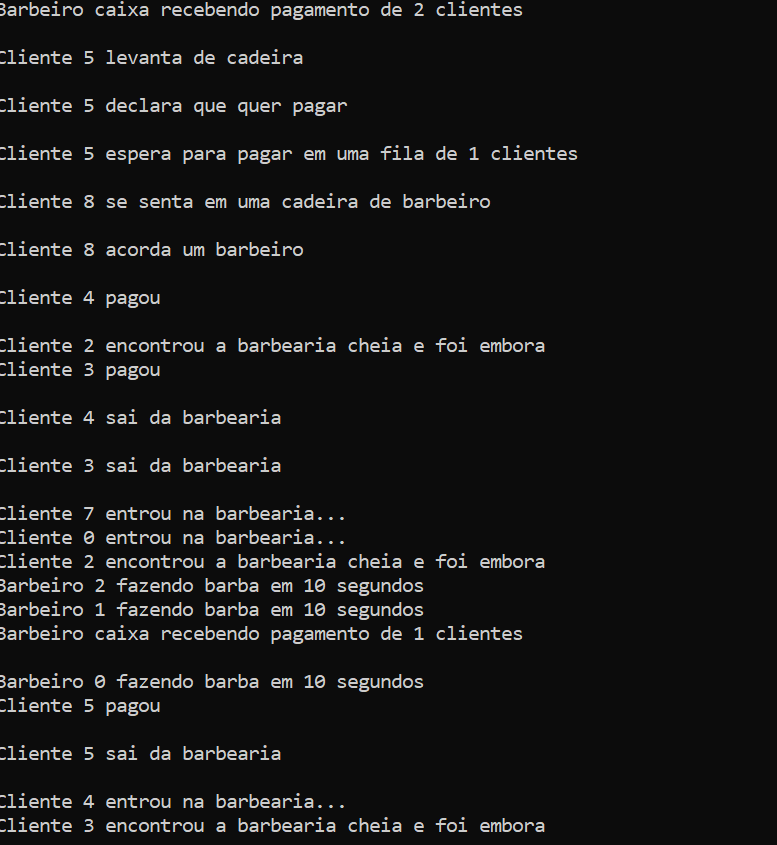
\includegraphics[scale=0.7]{10_clients.png}
    \caption{Caso para muitos (10) clientes}

\end{figure}

\begin{figure}[H]
    \centering
    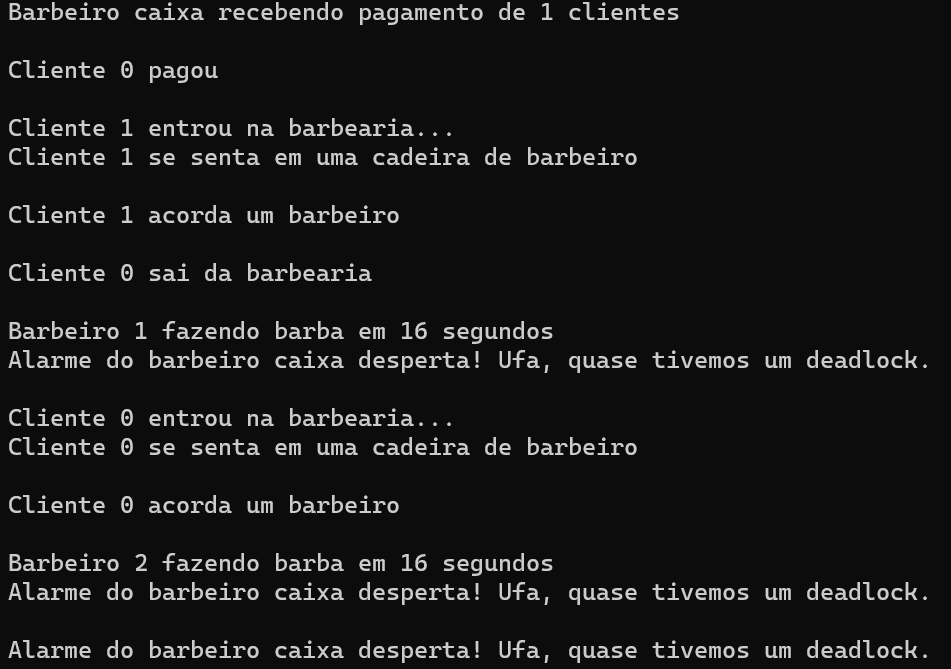
\includegraphics[scale=0.7]{2_clients.png}
    \caption{Caso para poucos clientes. Nota-se que o deadlock é evitado quase constantemente.}

\end{figure}

\begin{figure}[H]
    \centering
    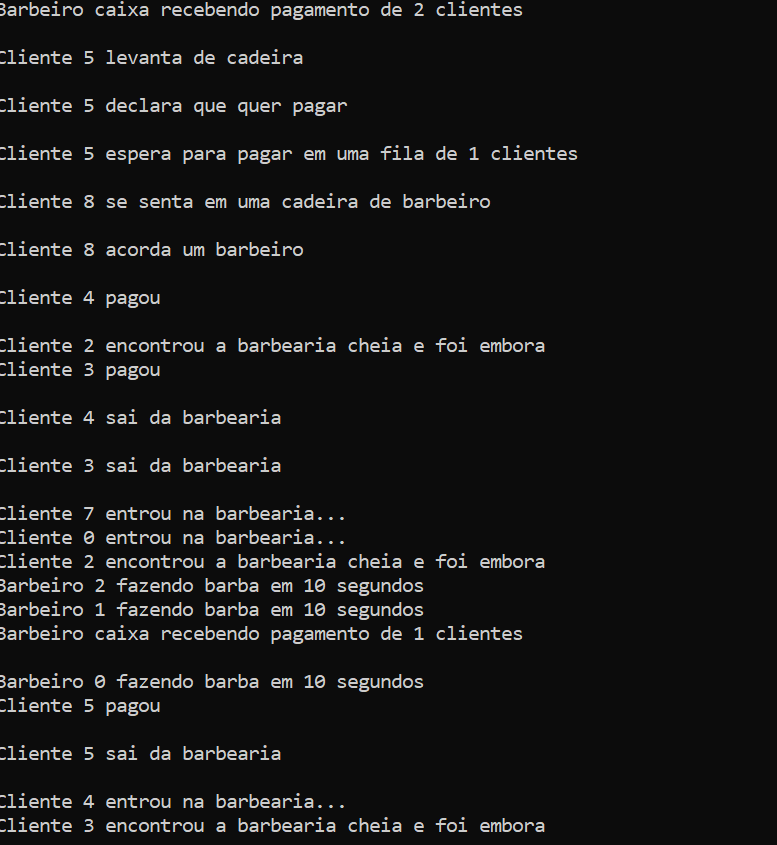
\includegraphics[scale=0.7]{10_clients.png}
    \caption{Caso para alguns (4) clientes}
 
\end{figure}

A reprodução desses experimentos garante observação que não há ocorrência de deadlock.

\section{Observações}

A solução proposta foi desenvolvida com o objetivo de funcionar de forma demonstrável e intuitiva. Sua implementação em algum contexto real levantaria preocupações sobre eficiência e justiça (\textit{fairness}) do atendimento (não há garantida da dinâmica FIFO nos semáforos da API utilizada).

\end{document}
